\section{Atividade 1 -- Encontrando Informações através do DNS}

\paragraph{}
Nesta atividade foram utilizadas as ferramentas \texttt{whois},
\texttt{dig} e \texttt{nslookup} para obtenção de informações relacionadas
a domínios e registros DNS.

\subsection{Pesquisa Reversa de IP com dig}

Foi executado o seguinte comando para realizar uma consulta reversa DNS
(\textit{Reverse DNS Lookup}):

\begin{verbatim}
dig -x 5.196.105.14
\end{verbatim}

\begin{figure}[H]
\centering
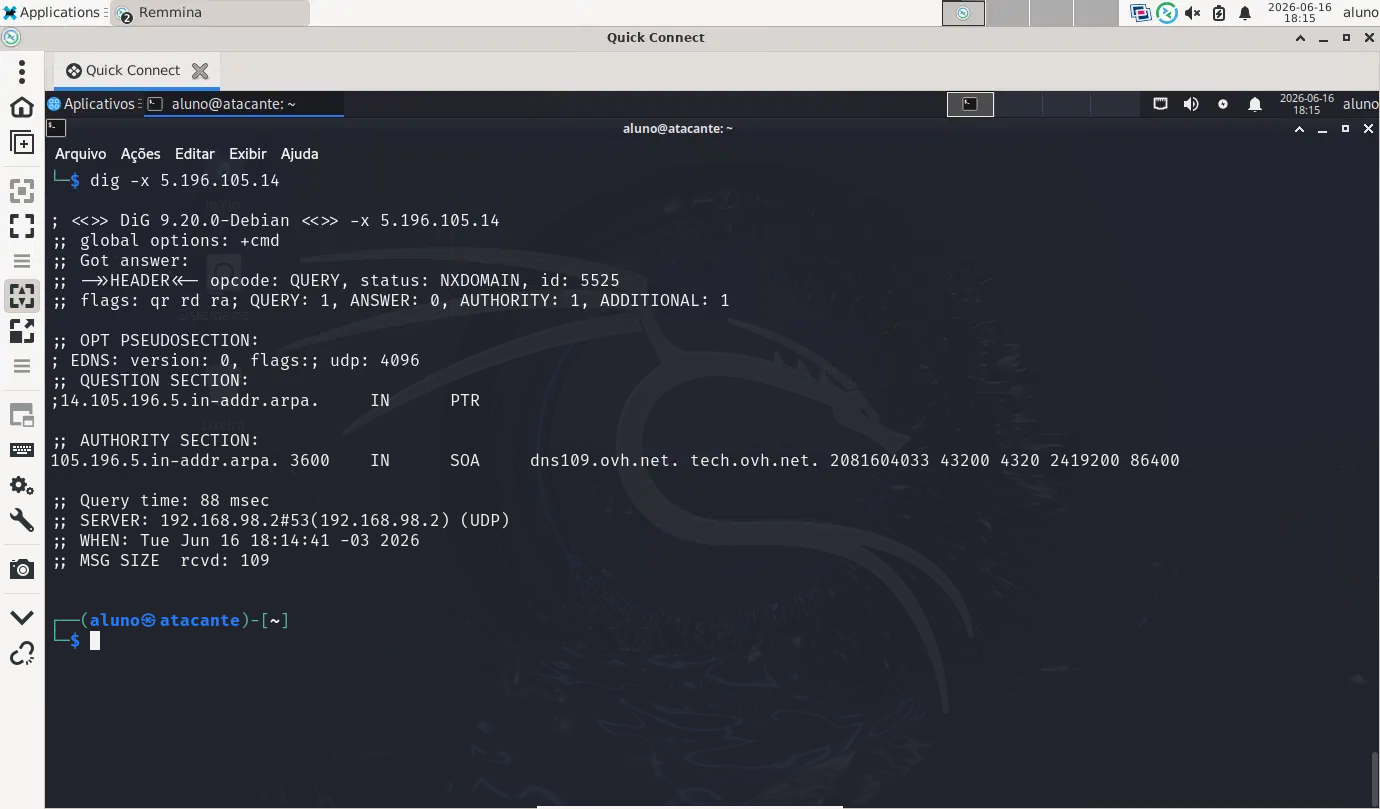
\includegraphics[width=0.95\textwidth]{./fig/atividade1-dig.png}
\caption{Resultado da pesquisa reversa utilizando o comando dig.}
\end{figure}

\paragraph{}
A consulta foi realizada para o endereço IP \texttt{5.196.105.14} com o
objetivo de identificar um possível registro PTR associado ao host.

\paragraph{}
O resultado retornou o status \texttt{NXDOMAIN} (\textit{Non-Existent Domain}),
indicando que não existe um registro PTR configurado para esse endereço IP na
zona reversa consultada. Dessa forma, não foi possível obter um nome de domínio
associado ao endereço analisado.

\paragraph{}
Além disso, a resposta apresentou informações da zona reversa administrada pela
OVH, incluindo o servidor DNS autoritativo \texttt{dns109.ovh.net}, responsável
pelas informações da faixa de endereços consultada.

\paragraph{}
A atividade permitiu compreender o funcionamento das consultas reversas DNS e a
importância dos registros PTR para identificação de hosts, análise de
infraestrutura e atividades de reconhecimento em processos de OSINT.
